% --- shared colours (matplotlib tab10) ---
\definecolor{cblue}{RGB}{31,119,180}
\definecolor{cred}{RGB}{214,39,40}
\definecolor{cgreen}{RGB}{44,160,44}

% common picture options: 1 bit = 0.042 cm on both axes (square aspect)
\tikzset{bitsec/.style={x=0.042cm,y=0.042cm,font=\small}}

%======================================================================
% PANEL 1 :  log t  vs  log eps   (advantage view)  --  SEARCH / linear
%======================================================================
\newcommand{\panelEpsSearch}{%
  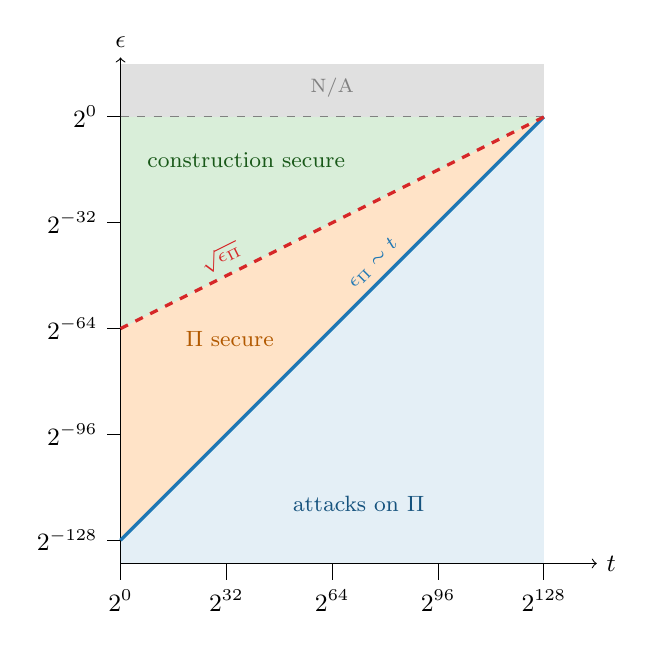
\begin{tikzpicture}[bitsec]
    \def\n{128}
    \fill[black!12]   (0,0) -- (0,16) -- (\n,16) -- (\n,0) -- cycle;
    \fill[cblue!12]  (0,-\n) -- (\n,0) -- (\n,-135) -- (0,-135) -- cycle;
    \fill[orange!22] (0,-\n) -- (0,{-\n/2}) -- (\n,0) -- cycle;
    \fill[cgreen!18] (0,{-\n/2}) -- (0,0) -- (\n,0) -- cycle;
    \draw[->] (0,-135) -- (0,18) node[above] {$\epsilon$};
    \draw[->] (0,-135) -- ({\n+16},-135) node[right] {$t$};
    \foreach \x in {0,32,64,96,128} \draw (\x,-135)--(\x,-140) node[below] {$2^{\x}$};
    \foreach \y in {0,-32,-64,-96,-128} \draw (0,\y)--(-4,\y) node[left] {$2^{\y}$};
    %\node[gray,rotate=90,anchor=south,font=\scriptsize] at (-24,-68) {$\downarrow$ more secure};
    \draw[gray,dashed] (0,0) -- (\n,0);
    \node[gray,font=\scriptsize] at ({0.5*\n},9) {N/A};
    \draw[cblue,very thick] (0,-\n) -- (\n,0);
    \draw[cred,very thick,dashed] (0,{-\n/2}) -- (\n,0);
    \node[cblue,rotate=45,anchor=south,font=\scriptsize] at (80,-48) {$\epsilon_\Pi \sim t$};
    \node[cred,rotate=26.57,anchor=south,font=\scriptsize] at (33,-48) {$\sqrt{\epsilon_\Pi}$};
    \node[cgreen!55!black,align=center,font=\footnotesize] at (38,-13) 
      {construction secure};
    \node[orange!70!black,align=center,font=\footnotesize] at (33,-67)
      %{primitive secure \\ construction broken?};
      {$\Pi$ secure};
    \node[cblue!70!black,align=center,font=\footnotesize] at (72,-117) 
      {attacks on $\Pi$};
  \end{tikzpicture}
}

%======================================================================
% PANEL 2 :  log t  vs  log eps   --  GROVER / collision
%======================================================================
\newcommand{\panelEpsGrover}{%
  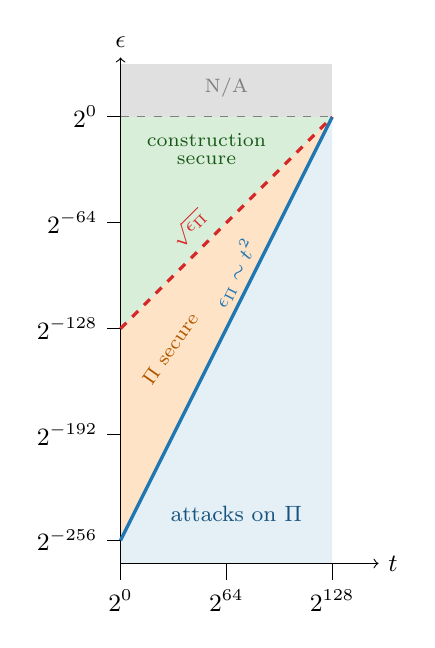
\begin{tikzpicture}[bitsec]
    \def\n{128}\def\m{64}
    \fill[black!12]   (0,0) -- (0,16) -- (\m,16) -- (\m,0) -- cycle;
    \fill[cblue!12]  (0,-\n) -- (\m,0) -- (\m,-135) -- (0,-135) -- cycle;
    \fill[orange!22] (0,-\n) -- (0,-\m) -- (\m,0) -- cycle;
    \fill[cgreen!18] (0,-\m) -- (0,0) -- (\m,0) -- cycle;
    \draw[->] (0,-135) -- (0,18) node[above] {$\epsilon$};
    \draw[->] (0,-135) -- ({\m+14},-135) node[right] {$t$};
    \foreach \x in {0,64,128} \draw ({\x/2},-135)--({\x/2},-140) node[below] {$2^{\x}$};
    \foreach \y in {0,-64,-128,-192,-256} \draw (0,{\y/2})--(-4,{\y/2}) node[left] {$2^{\y}$};
    \draw[gray,dashed] (0,0) -- (\m,0);
    \node[gray,font=\scriptsize] at (32,9) {N/A};
    \draw[cblue,very thick] (0,-\n) -- (\m,0);
    \draw[cred,very thick,dashed] (0,-\m) -- (\m,0);
    \node[cblue,rotate=63.43,anchor=south,font=\scriptsize] at (40,-50) {$\epsilon_\Pi \sim t^2$};
    \node[cred,rotate=45,anchor=south,font=\scriptsize] at (25,-38) {$\sqrt{\epsilon_\Pi}$};
    \node[cgreen!55!black,align=center,font=\scriptsize] at (26,-7) {construction};
    \node[cgreen!55!black,align=center,font=\scriptsize] at (26,-13) {secure};
    \node[orange!70!black,align=center,rotate=55,font=\scriptsize] at (15,-70) {$\Pi$ secure};
    \node[cblue!70!black,align=center,font=\footnotesize] at (35,-120) {attacks on $\Pi$};
  \end{tikzpicture}
}

%======================================================================
% PANEL 3 :  log t  vs  log eps   --  Quantum collision search
%======================================================================
\newcommand{\panelEpsCube}{%
  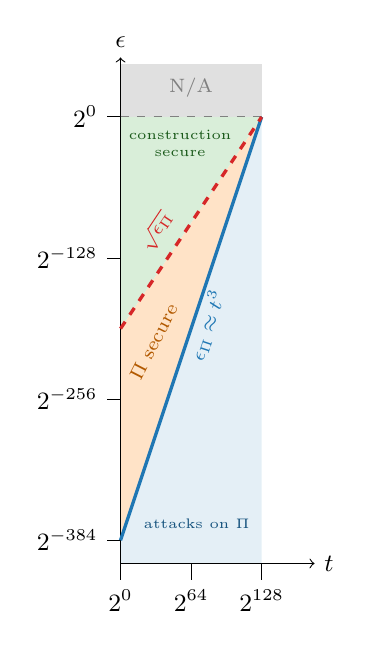
\begin{tikzpicture}[bitsec]
    \def\n{128}% depth 128 drawn = 384 bits; pinch x = \n/3
    \fill[black!12]  (0,0) -- (0,16) -- ({\n/3},16) -- ({\n/3},0) -- cycle;
    \fill[cblue!12]  (0,-\n) -- ({\n/3},0) -- ({\n/3},-135) -- (0,-135) -- cycle;
    \fill[orange!22] (0,-\n) -- (0,{-\n/2}) -- ({\n/3},0) -- cycle;
    \fill[cgreen!18] (0,{-\n/2}) -- (0,0) -- ({\n/3},0) -- cycle;
    \draw[->] (0,-135) -- (0,18) node[above] {$\epsilon$};
    \draw[->] (0,-135) -- ({\n/3+16},-135) node[right] {$t$};
    \foreach \x in {0,64,128} \draw ({\x/3},-135)--({\x/3},-140) node[below] {$2^{\x}$};
    \foreach \y in {0,-128,-256,-384} \draw (0,{\y/3})--(-4,{\y/3}) node[left] {$2^{\y}$};
    \draw[gray,dashed] (0,0) -- ({\n/3},0);
    \node[gray,font=\scriptsize] at ({\n/6},9) {N/A};
    \draw[cblue,very thick] (0,-\n) -- ({\n/3},0);
    \draw[cred,very thick,dashed] (0,{-\n/2}) -- ({\n/3},0);
    \node[cblue,rotate=71.57,anchor=south,font=\scriptsize] at (32,-65) {$\epsilon_\Pi \approx t^3$};
    \node[cred,rotate=56.31,anchor=south,font=\scriptsize] at (16,-38) {$\sqrt{\epsilon_\Pi}$};
    \node[cgreen!55!black,align=center,font=\tiny] at (18,-8) {construction\\secure};
    \node[orange!70!black,align=center,rotate=63,font=\scriptsize] at (10,-68) {$\Pi$ secure};
    \node[cblue!70!black,align=center,font=\tiny] at (23,-123) {attacks on $\Pi$};
  \end{tikzpicture}
}

%======================================================================
% PANEL 4 :  t  vs  kappa   (bit-security view)  --  SEARCH / linear
%======================================================================
\newcommand{\panelKapSearch}{%
  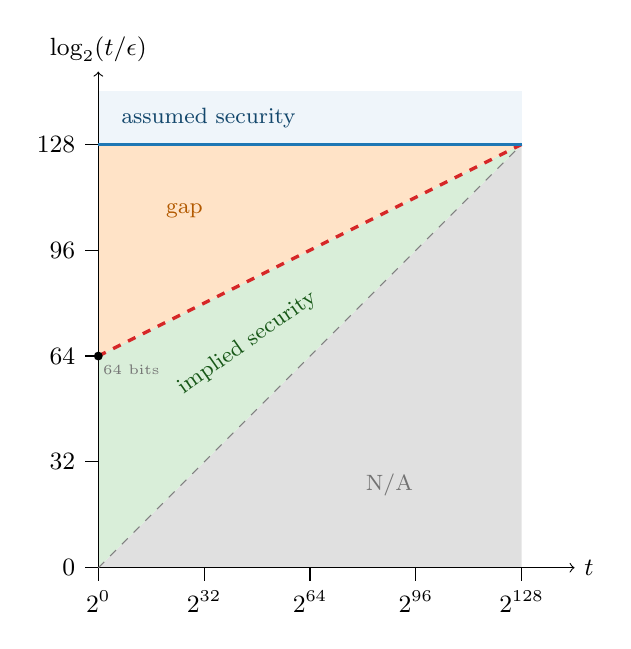
\begin{tikzpicture}[bitsec]
    \def\n{128}
    \fill[cblue!7]   (0,\n) -- (0,{\n+16}) -- (\n,{\n+16}) -- (\n,\n) -- cycle;
    \fill[black!12]  (0,0) -- (\n,\n) -- (\n,0) -- cycle;
    \fill[cgreen!18] (0,0) -- (0,{\n/2}) -- (\n,\n) -- cycle;
    \fill[orange!22] (0,{\n/2}) -- (0,\n) -- (\n,\n) -- cycle;
    \draw[->] (0,0) -- (0,{\n+22}) node[above] {$\log_2(t/\epsilon)$};
    \draw[->] (0,0) -- ({\n+16},0) node[right] {$t$};
    \foreach \x in {0,32,64,96,128} \draw (\x,0)--(\x,-4) node[below] {$2^{\x}$};
    \foreach \y in {0,32,64,96,128} \draw (0,\y)--(-4,\y) node[left] {$\y$};
    \draw[gray,dashed] (0,0) -- (\n,\n);
    \draw[cred,very thick,dashed] (0,{\n/2}) -- (\n,\n);
    \draw[cblue,very thick] (0,\n) -- (\n,\n);
    \fill (0,64) circle (1.6pt);
    \node[black!55,font=\tiny] at (10,60) {$64$ bits};
    %\node[gray,rotate=45,anchor=south,font=\footnotesize] at (104,104) {$\epsilon=1$};
    %\node[cred,rotate=26.57,anchor=south,font=\footnotesize] at (58,90) {$\kappa_A=\tfrac12(\tau+n)$};
    %\node[cblue,anchor=south,font=\footnotesize] at (96,129) {$\kappa_B=n$};
    \node[cblue!60!black,anchor=west,font=\footnotesize] at (4,{\n+8}) {assumed security};
    \node[orange!70!black,font=\footnotesize] at (26,108) {gap};
    \node[cgreen!55!black,rotate=35,font=\footnotesize] at (45,68) {implied security};
    \node[black!55,align=center,font=\footnotesize] at (88,25) {N/A};
  \end{tikzpicture}
}

%======================================================================
% PANEL 5 :  t  vs  kappa   --  GROVER / collision
%======================================================================
\newcommand{\panelKapGrover}{%
  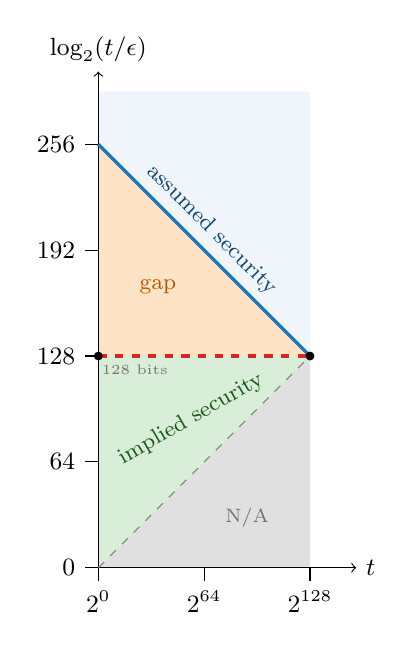
\begin{tikzpicture}[bitsec]
    \def\n{128}\def\m{64}
    \fill[cblue!7]   (0,\n) -- (0,{\n+16}) -- (\m,{\n+16}) -- (\m,\m) -- cycle;
    \fill[black!12]  (0,0) -- (\m,\m) -- (\m,0) -- cycle;
    \fill[cgreen!18] (0,0) -- (0,\m) -- (\m,\m) -- cycle;
    \fill[orange!22] (0,\m) -- (0,\n) -- (\m,\m) -- cycle;
    \draw[->] (0,0) -- (0,{\n+22}) node[above] {$\log_2(t/\epsilon)$};
    \draw[->] (0,0) -- ({\m+14},0) node[right] {$t$};
    \foreach \x in {0,64,128} \draw ({\x/2},0)--({\x/2},-4) node[below] {$2^{\x}$};
    \foreach \y in {0,64,128,192,256} \draw (0,{\y/2})--(-4,{\y/2}) node[left] {$\y$};
    \draw[gray,dashed] (0,0) -- (\m,\m);
    \draw[cblue,very thick] (0,\n) -- (\m,\m);
    \draw[cred,very thick,dashed] (0,\m) -- (\m,\m);
    \fill (0,\m) circle (1.6pt);
    \fill (\m,\m) circle (1.6pt);
    \node[black!55,font=\tiny] at (11,60) {$128$ bits};
    %\node[cblue,rotate=-45,anchor=south,font=\footnotesize] at (24,104) {$\kappa_B=n-\tau$};
    %\node[cred,anchor=south,font=\footnotesize] at (18,65) {$\kappa_A=n/2$};
    %\node[gray,rotate=45,anchor=south,font=\footnotesize] at (28,28) {$\epsilon=1$};
    \node[cblue!60!black,rotate=-45,anchor=south,font=\footnotesize] at (30,98) {assumed security};
    \node[orange!70!black,font=\footnotesize] at (18,85) {gap};
    \node[cgreen!55!black,rotate=30,font=\footnotesize] at (28,45) {implied security};
    \node[black!55,font=\scriptsize] at (45,15) {N/A};
  \end{tikzpicture}
}

%======================================================================
% PANEL 6 :  t  vs  kappa   --  Quantum collision search
%======================================================================
\newcommand{\panelKapCube}{%
  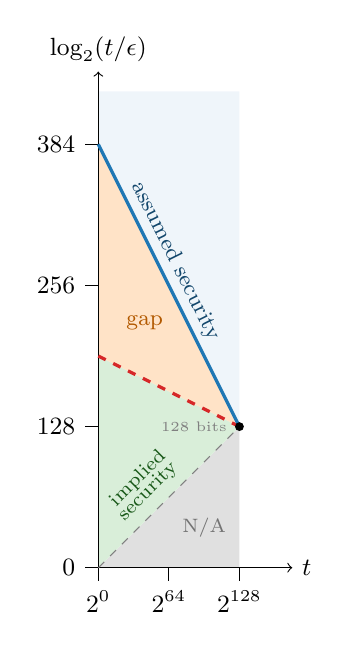
\begin{tikzpicture}[bitsec]
    \def\n{128}
    \fill[cblue!7]   (0,\n) -- (0,{\n+16}) -- ({\n/3},{\n+16}) -- ({\n/3},{\n/3}) -- cycle;
    \fill[black!12]  (0,0) -- ({\n/3},{\n/3}) -- ({\n/3},0) -- cycle;
    \fill[cgreen!18] (0,0) -- (0,{\n/2}) -- ({\n/3},{\n/3}) -- cycle;
    \fill[orange!22] (0,{\n/2}) -- (0,\n) -- ({\n/3},{\n/3}) -- cycle;
    \draw[->] (0,0) -- (0,{\n+22}) node[above] {$\log_2(t/\epsilon)$};
    \draw[->] (0,0) -- ({\n/3+16},0) node[right] {$t$};
    \foreach \x in {0,64,128} \draw ({\x/3},0)--({\x/3},-4) node[below] {$2^{\x}$};
    \foreach \y in {0,128,256,384} \draw (0,{\y/3})--(-4,{\y/3}) node[left] {$\y$};
    \draw[gray,dashed] (0,0) -- ({\n/3},{\n/3});
    \draw[cred,very thick,dashed] (0,{\n/2}) -- ({\n/3},{\n/3});
    \draw[cblue,very thick] (0,\n) -- ({\n/3},{\n/3});
    \fill ({\n/3},{\n/3}) circle (1.6pt);
    \node[anchor=west,font=\tiny,gray] at (16,{\n/3}) {128 bits};
    \node[cblue!60!black,rotate=-63.43,anchor=south,font=\footnotesize] at (18,90) {assumed security};
    \node[orange!70!black,font=\footnotesize] at (14,74) {gap};
    \node[cgreen!55!black,rotate=45,font=\scriptsize] at (12,27) {implied};
    \node[cgreen!55!black,rotate=45,font=\scriptsize] at (15,23) {security};
    \node[black!55,font=\scriptsize] at (32,12) {N/A};
  \end{tikzpicture}
}

%%% Invoking the Panels as Sub-Figures %%%
% Fixed scale + tabular  =>  Grover panel is literally half as wide,
% and the two x-axes align on a common baseline automatically.
%\begin{tabular}{@{}c@{\hspace{3em}}c@{}}
%  \panelEpsSearch & \panelEpsGrover\\[3pt]
%  {\small (a) Attack space if best primitive attack $=$ brute-force} & {\small (b) Attack space if best primitive attack $=$ Grover}\\[8pt]
%  \panelKapSearch & \panelKapGrover\\[3pt]
%  {\small (c) Bit security if best primitive attack $=$ brute-force} & {\small (d) Bit security if best primitive attack $=$ Grover}\\
%\end{tabular}

\resizebox{\textwidth}{!}{
  \begin{tabular}{@{}c@{\hspace{1em}}c@{\hspace{1em}}c@{}}
    \panelcap{\panelEpsSearch}{
      %(a) Possible attacks if best attack against the
      %primitive scales linearly with time (brute-force)
      (a) Ruled-out attacks if the best attack on the primitive scales
      \emph{linearly} (brute-force)
    }
    & \panelcap{\panelEpsGrover}{
      (b) vs.\ \emph{quadratically} (birthday/Grover)
    } 
    & \panelcap{\panelEpsCube}{
      (c) vs.\ \emph{qubically} \\ (Quantum coll.)
    } \\[30pt]
    \panelcap{\panelKapSearch}{
      %(c) Bit security if best primitive attack $=$ brute-force
      (d) Bit security if the best attack on the primitive scales
      \emph{linearly} (brute-force)
    }
    & \panelcap{\panelKapGrover}{
      (e) vs.\ \emph{quadratically} (birthday/Grover)
    }
    & \panelcap{\panelKapCube}{
      (f) vs.\ \emph{qubically} \\ (Quantum coll.)
    } \\[30pt]
  \end{tabular}
}
